%% ----------------------------------------------------------------------------
% CVG SA/MA thesis template
%
% Created 03/08/2024 by Tobias Fischer
%% ----------------------------------------------------------------------------
\newpage
\chapter{Experiments}

[We prepare x different question datasets to experiment on: 1) easy 2) hard 3) complete/mixed 4) constant scenes]

In this section, we detail experimental methods and results for the generation of the ScanSG dataset and the proposed ScanSG-Transformer model.

\section{Scene Graph Generation}

[Note: we remove scenes with segmentation errors (some segmented objects do not appear in any of the images -- specifically scenes 180, 279, 305, 530, 597)]

In order to train a successful 3D-VQA model, we must ensure that its input data, namely generated scene graphs and questions, are of high quality. This section empirically evaluates the impact of different design choices on the quality of the generated scene graphs. We evaluate the design choices for scene graph nodes and edges separately, and choose the best performing parameters for the proposed scene graph dataset. For scene graph nodes, we evaluate the effects of different cropping methods, k-values, and visibility scores on the quality of the node embeddings. For scene graph edges, we evaluate the impact of different threshold values on the quality of the edges in the scene graphs.

All experiments in this section are performed on a smaller subset of the dataset, consisting of 71 scenes, with a total of 2467 objects across scenes. This subset is also used for testing in section XXX.

\subsection{Node Construction}
We evaluate the impact of different cropping methods, k-values and visibility scores on the quality of the generated node CLIP-embeddings. The following paragraphs detail the methods and parameters considered for each of these design choices.

\bigskip \noindent
\textbf{Cropping method:}
We compare the impact of the following cropping methods on node embedding quality (illustrated in Figure XXX):
\begin{enumerate}
    \item A tight, rectangular crop around the object with all background pixels masked out. With this method, the object is centered in the image, and the background is removed. However, CLIP was trained on square images with no background removal. To adapt rectangular crops to CLIP, we use the resizing method described in the original CLIP paper [XXX]: the crop is resized to $224$ in its minimum dimension, and then randomly cropped to a $224 \times 224$ square.
    
    \item A tight, rectangular crop around the object with no further changes. With this method, the object is centered in the image. However, the background is not removed, meaning other surrounding objects could contribute to the embedding, and the image is not square. The rectangular crops are resized as in the original CLIP paper [XXX].
    
    \item A square crop centred around the object, resized to $224 \times 224$. With this method, the crop is square and correctly sized, and no further processing is needed. However, the background is not removed and the non-tight crop means other surrounding objects might contribute to the node embedding.
    
    \item A tight, rectangular crop, resized to $224 \times 224$. With this method, the crop is tight around the object (fewer surrounding objects included in the crop). However, the resized crops distort the image, and CLIP was not trained on distorted images.
\end{enumerate}

\begin{figure}[h!]
    \centering
    \begin{minipage}[b]{0.1\textwidth}
        \centering
        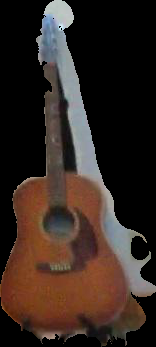
\includegraphics[width=\textwidth]{images/cropping_method_0.png}
        \caption{Caption 1}
    \end{minipage}
    \hspace{1em} % Adjust this to control the horizontal space between images
    \begin{minipage}[b]{0.1\textwidth}
        \centering
        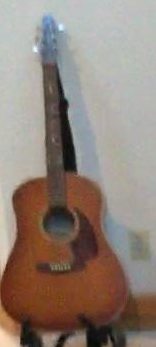
\includegraphics[width=\textwidth]{images/cropping_method_1.png}
        \caption{Caption 2}
    \end{minipage}
    \vspace{0em} % Adjust this to control the vertical space between rows
    \begin{minipage}[b]{0.1\textwidth}
        \centering
        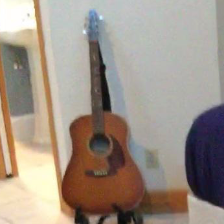
\includegraphics[width=\textwidth]{images/cropping_method_2.png}
        \caption{Caption 3}
    \end{minipage}
    \hspace{1em} % Adjust this to control the horizontal space between images
    \begin{minipage}[b]{0.1\textwidth}
        \centering
        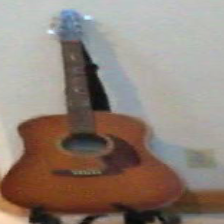
\includegraphics[width=\textwidth]{images/cropping_method_3.png}
        \caption{Caption 4}
    \end{minipage}
    \caption{Overall figure caption}
\end{figure}

\bigskip \noindent
\textbf{k-value:}
We also evaluate the impact of different k-values on the quality of the scene graph nodes. The k-value determines how many images of the object will be considered when generating the scene graph node. A higher value of k could result in a more accurate representation of the object, but could also introduce noise or inconsistencies as different views may have different different embeddings. We not that increasing the k-value highly increases the computational cost. It is therefore important to find the optimal k-value that balances these trade-offs. In this analysis we consider the following k-values: $k=1$, $k=3$, and $k=10$.

\bigskip \noindent
\textbf{Visibility score:}
\begin{enumerate}
    \item $s_1 = \frac{n}{w \times h} \times \frac{b}{8}$
    \item $s_2 = w_p \frac{n}{w \times h} + w_c \frac{b}{8}$ with $w_p = 1$, $w_c = 1$
    \item $s_2$ with $w_p = 100$, $w_c = 1$
    \item $s_2$ with $w_p = 1$, $w_c = 100$
\end{enumerate}

To evaluate the comparative quality of these cropping methods and k-values, we perform the following experiment: first, we generate scene graphs using each of the three cropping methods, with $k=1$, $k=3$ and $k=10$ respectively. We therefore have a total of 9 different scene graph node generation methods. Then, we CLIP-embed all the object labels in the scene, and calculate the similarity between the embeddings of the object crops and the embeddings of the object labels. For each object, we select the label with the highest similarity, and compare it to the ground truth label. We calculate the accuracy of the scene graph nodes for each of the 9 methods, and choose the best performing method for the final model.  Note that we only use semantic accuracy (since there is no context-awareness mechanism or learning in this experiment) to evaluate the quality of the scene graph nodes. The semantic accuracy is the percentage of nodes that are embedded closest to their label in the CLIP embedding space. We repeat this experiment for each visibility score listed above, keeping the cropping method and k-value constant. Tables XX shows the results of this experiment.

\begin{table}[h!]
    \centering
    \caption{}
    \begin{tabular}{l|lll|}
    \cline{2-4}
                                                   & \multicolumn{3}{c|}{\textbf{k-value}} \\ \hline
    \multicolumn{1}{|c|}{\textbf{Cropping method}} & 1        & 3       & 10               \\ \hline
    \multicolumn{1}{|l|}{Tight masked crop}        & 49.5     & 50.1    & 52.1             \\
    \multicolumn{1}{|l|}{Tight crop}               & 57.6     & 58.9    & 60.3             \\
    \multicolumn{1}{|l|}{Square crop}              & 57.1     & 58.3    & \textbf{62.2}    \\
    \multicolumn{1}{|l|}{Tight resized crop}       & 56.2     & 57.4    & 60.2             \\ \hline
    \end{tabular}
\end{table}
\begin{table}[h!]
    \centering
    \caption{}
    \begin{tabular}{|c|c|}
    \hline
    \textbf{Visibility Score} & \textbf{Accuracy} \\ \hline
    s1                       & 62.2               \\ \hline
    s2                        & 78.2                  \\ \hline
    s3                        &                   \\ \hline
    s4                        &                   \\ \hline
    \end{tabular}
\end{table}

\bigskip
\noindent
\textbf{Results and Interpretation}

Table XX shows some examples of inaccurate node embeddings. The table shows the crop of the object, the ground truth label, and the label with the highest similarity to the object crop. These inaccuracies are most often caused by other objects appearing in the object of interest's crop for the following reasons:
\begin{itemize}
    \item they occlude the object of interest (see floor example)
    \item they are contained within the object of interest (see doorframe example)
    \item they are similar to the object of interest (see shelf example)
    \item the object of interest is rectangular so a square crop includes other objects (see guitar case example)
\end{itemize}

\begin{table}[h]
    \centering
    \caption{\textcolor{red}{add the GT and pred label under each image, show them all side by side.}}
    \begin{tabular}{|c|l|l|}
        \hline
        \textbf{Crop} & \textbf{Ground Truth Label} & \textbf{Most Similar Label} \\ \hline
        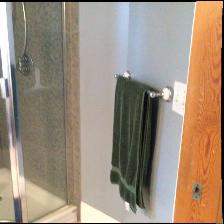
\includegraphics[width=1in]{images/wall.png} & Wall & Shower \\ \hline
        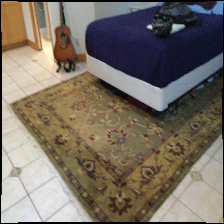
\includegraphics[width=1in]{images/floor.png} & Floor & Bed \\ \hline
        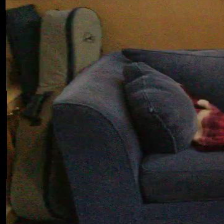
\includegraphics[width=1in]{images/guitar case.png} & Guitar Case & Couch \\ \hline
        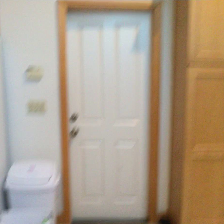
\includegraphics[width=1in]{images/doorframe.png} & Doorframe & Door \\ \hline
        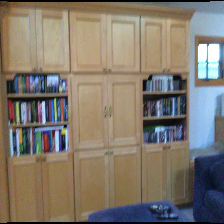
\includegraphics[width=1in]{images/shelf.png} & Shelf & Cabinet \\ \hline
    \end{tabular}
\end{table}

These examples highlight some inherent limitations of the CLIP method. However, we believe CLIP embeddings are still a good starting points as they offer a common embedding for the images in text, which is accurate in most cases.

\textcolor{red}{showcases some of the important clip limitations. we further discuss these limitations in Section XX (Discussion). }

The experiments also highlight the necessity of including some learning into the model, because the CLIP-embedding of the object is not very close to the CLIP-embedding of the object label. And this label task is easier than the question task, as shown in Figure XXX.


\subsection{Edge Construction}
Same model, same node embeddings (only change is the edges).

\begin{table}[h!]
    \centering
    \caption{accuracy (percent)}
    \begin{tabular}{|c|c|}
    \hline
    \multicolumn{1}{|l|}{\textbf{Threshold value (m)}} & \textbf{EM@1 (\%)} \\ \hline
    0.2                                                & \textbf{20.1}      \\ \hline
    0.5                                                & 14.6               \\ \hline
    0.8                                                & 9.8                \\ \hline
    Random edges                                       & 4.0                \\ \hline
    \end{tabular}
    \end{table}

Dense graphs perform better than sparse graphs. Cannot use no edges because then the scene structure is lost.
So these edges help the model learn.

We train GNN model on the scene graphs with different threshold values for the edges. We evaluate the performance of the model on the test set, and choose the best threshold value for the final sg dataset. We also compare the performance of the model with the best threshold value to the performance of the model with random edges. Table XXX shows the results of this experiment.

Simple GNN model -> show that chosen threshold is better than random edges.
Also show that edges can have a huge impact on the final answer --> must be chosen carefully.



\subsection{Edge Label Classification}

\subsection{Dataset Statistics}
(Add to appendix instead)
Average number of edges per graph, "impact window"? ...


%%%%%%%%%%%%%%%%%%%%%%%%%%%%%%%%%%%% VQA %%%%%%%%%%%%%%%%%%%%%%%%%%%%%%%%%%

\section{Visual Question Answering Model}

In this section, we assess the performance of each model described in section XXX on the generated ScanSG dataset. The evaluation metrics and hyperparameters common to all experiments are described below. The details specific to each experiment are described in the relevant sections, such that the results can be reproduced.

\textcolor{red}{
Our model introduces 2 new components compared to the traditional baseline: edge information + cross-attention. This section investigates the added benefit of each component in the context of the ScanSG + ScanQA dataset.}

\textcolor{red}{
Turns out cross attention definitely contributes to higher performance (the ScanSG-noGNN always outperforms the baseline). The GNN does not actually contribute, but this is most likely because it is not suited to this dataset. this dataset contains very little data which can actually take advantage of the gnn structure. In conclusion, this is the best we can do with the data we have. Need better Q dataset (maybe one that lists all possible answers!!), and maybe need to think of other ways to embed the nodes (such as owl?).
}

\subsection{GraphVQA}
\textcolor{red}{
what we tried, the results were random on the scenes tested.
the main issue was that this method relies on the "programs" but we had none for this method.
so this is also a sign that the model was overfit to their specific dataset.}

\subsection{Experimental Setup}

\bigskip
\noindent \textbf{Dataset}
The test/train split from the original ScanQA paper [XXX] is used. Multi-answer questions are removed such that each question has exactly one answer. Unless otherwise stated, the training set consits of $92\%$ of the dataset with 19,500 questions about 555 scenes. The test set consists of the remaining $8\%$ with 1,581 questions about 71 scenes. The scenes in the training and test set are kept separate, such that during testing, the model sees new questions about unseen scenes.

\bigskip
\noindent \textbf{Hyperparameters}
For the baseline model, no training is required, hence none of the following hyperparameters are relevant. For all other models, a batch size of $64$ was used for all experiments. The Adam optimizer was used with a learning rate tuned to each model. The loss function used was the cross-entropy loss, except if stated otherwise. The models were trained for $200$ epochs.

\bigskip
\noindent \textbf{Evaluation metrics}
We compare the performance of each model on the test set of the ScanSG dataset, and report the results in terms of best EM@1 (same as instance accuracy), EM@5 and EM@10 achieved. EM@K is the percentage of questions for which the correct answer is in the top-K predicted answers. We report three measures of EM@K to understand the performance at different levels of accuracy, and monitor these metrics during training to understand how the models learn. An increasing EM@10 score indicates that the model is learning to predict the correct answer with higher confidence, while an increasing EM@1 score indicates that the model is learning to predict the correct answer with higher accuracy. We also report the semantic accuracy, Sem-EM@1. The semantic accuracy indicates correct label prediction, regardless of predicted instance. A high discrepancy between EM@1 and Sem-EM@1 indicates that the model correctly identifies the answer label, but struggles to identify the correct instance of this label. Table XXX summarizes the results achieved by each model.

\bigskip
\noindent \textbf{Loss function}
The cross-entropy loss is used across all experiments, unless stated otherwise.

\subsection{Model Performance on ScanSG + ScanQA}

Table XX shows the performance of each model on the generated ScanSG+ScanQA dataset.

\begin{table}[h!]
    \centering
    \caption{Performance on the full ScanSG+ScanQA dataset, with node embeddings computed from the top-k image crops, as described in XX.}
    \begin{tabular}{|l|c|c|c|c|}
    \hline
    \textbf{Model}         & \textbf{EM@1} & \textbf{EM@5} & \textbf{EM@10} & \textbf{Sem-EM@1} \\ \hline
    Baseline               & 28.1 & 59.7 & 73.8 & 36.4  \\ \hline
    Baseline + GNN         & 12.3 & 38.8 & 54.3 & 18.9  \\ \hline
    ScanSG-GNN             & 25.3 & 64.2 & 81.2 & 33.5 \\ \hline
    ScanSG-noGNN           & \textbf{43.6} & \textbf{73.9} & \textbf{86.6} & \textbf{55.7} \\ \hline
    \end{tabular}
\end{table}

\bigskip \noindent
\textbf{Baseline}
Since the baseline model does not require any training, it is simply evaluated on the test set of the ScanSG dataset. The hyperparameters and loss function are irrelevant.

The baseline model does not utilize edge information (which encodes scene structure and 3D information), and thus does not have the ability to differentiate between instances of the same object class. This results in a higher semantic accuracy (Sem-EM@1) than instance accuracy (EM@1), as seen in Table XX.

Furthermore, since the baseline relies on static, pre-computed text and image embeddings, it cannot learn from the data. While this makes the baseline a highly generalisable model, it also means that the model performs poorly on samples where CLIP(question) has a dissimilar pre-computed embedding than CLIP(answer). Since CLIP was trained on descriptive captions rather than questions about the image, it is expected that question embeddings may not align with their associated answer.


\bigskip \noindent
\textbf{Baseline + GNN}
\textcolor{red}{Learning rate for Baseline + GNN:}

The Basline+GNN model adds a learning component to the Baseline model, in the form of a GCN which propagates node information to its neighbours, such that each node gains an awareness of its surroundings. This makes for a context-aware scene representation.

However, Table XX shows that this method performs worse than the simple baseline. This can be explained by the fact that the Baseline + GNN model computes the cosine similarity between a dynamic, learnable embedding (nodes) and a static, pre-computed embedding (question). This method incentivises the model to update node embeddings such that they better align with the questions they answer. However, as some questions have the same answer but very different embeddings, this creates conflicting training examples. Noisy data impedes model learning.

\textcolor{red}{+ maybe add a figure to illustrate this}

\textcolor{red}{+ also maybe not enough data that actually needs a gnn. pull these two conclusions together in the final conclusion}

\bigskip \noindent
\textbf{ScanSG-GNN}
The ScanSG-GNN model adds learnable, word-level text embeddings, and a cross-attention mechanism. The performance of this model is similar to that of the basline model, but with higher confidence (higher EM@5 and EM@10 scores than the baseline).

\bigskip \noindent
\textbf{ScanSG-noGNN}
This model is the ScanSG-GNN model stripped of the GNN. The difference between ScanSG-noGNN and the baseline is that there is word-level embedding and a cross-attention mechanism.

This model outperforms the ScanSG-GNN model. However, since it has been stripped of the GNN, it has no context awareness (two scenes with the same objects in different positions would have the same encoding), and should not be able to answer relational questions. This means that the model is not learning the scene structure but rather language priors.

This model performs the best, indicating that the cross-attention mechanism with the word-level embeddings work better than the cosine similarity of embeddings. This also indicates that the GNN does not benefit model performance.

\bigskip
\noindent
We note that all models display strong overfitting. \textcolor{red}{add proof in appendix.}
In the following section, we address the following questions, which arise from the experiment: 1) Can we regularize the ScanSG model to prevent overfitting? 2) Can the overfitting be explained by poor data quality? and 3) Why does the GNN component decrease accuracy?

\textcolor{red}{likely because the gnn is data hungry and there is not that much data that requires information propagation. the hard questions do but also they are likely too hard (even for human, they have many possible answers).}


\subsection{Addressing Overfitting}
The discrepancy between the train and test accuracy (and loss) suggests that the models suffer from overfitting. This is further illustrated in Figures XXX. While the train accuracy increases with increasing number of training epochs, the test accuracy initially increases, and starts to decrease after around 6 epochs. In Figure XXX, the train loss decreases with increasing number of epochs, whereas the test loss initially decreases, and then starts to increase around 6 epochs. This indicates that the model is overfitting to the training data, limiting its generalization to the test data.

% \begin{figure}[h!]
%     \centering
%     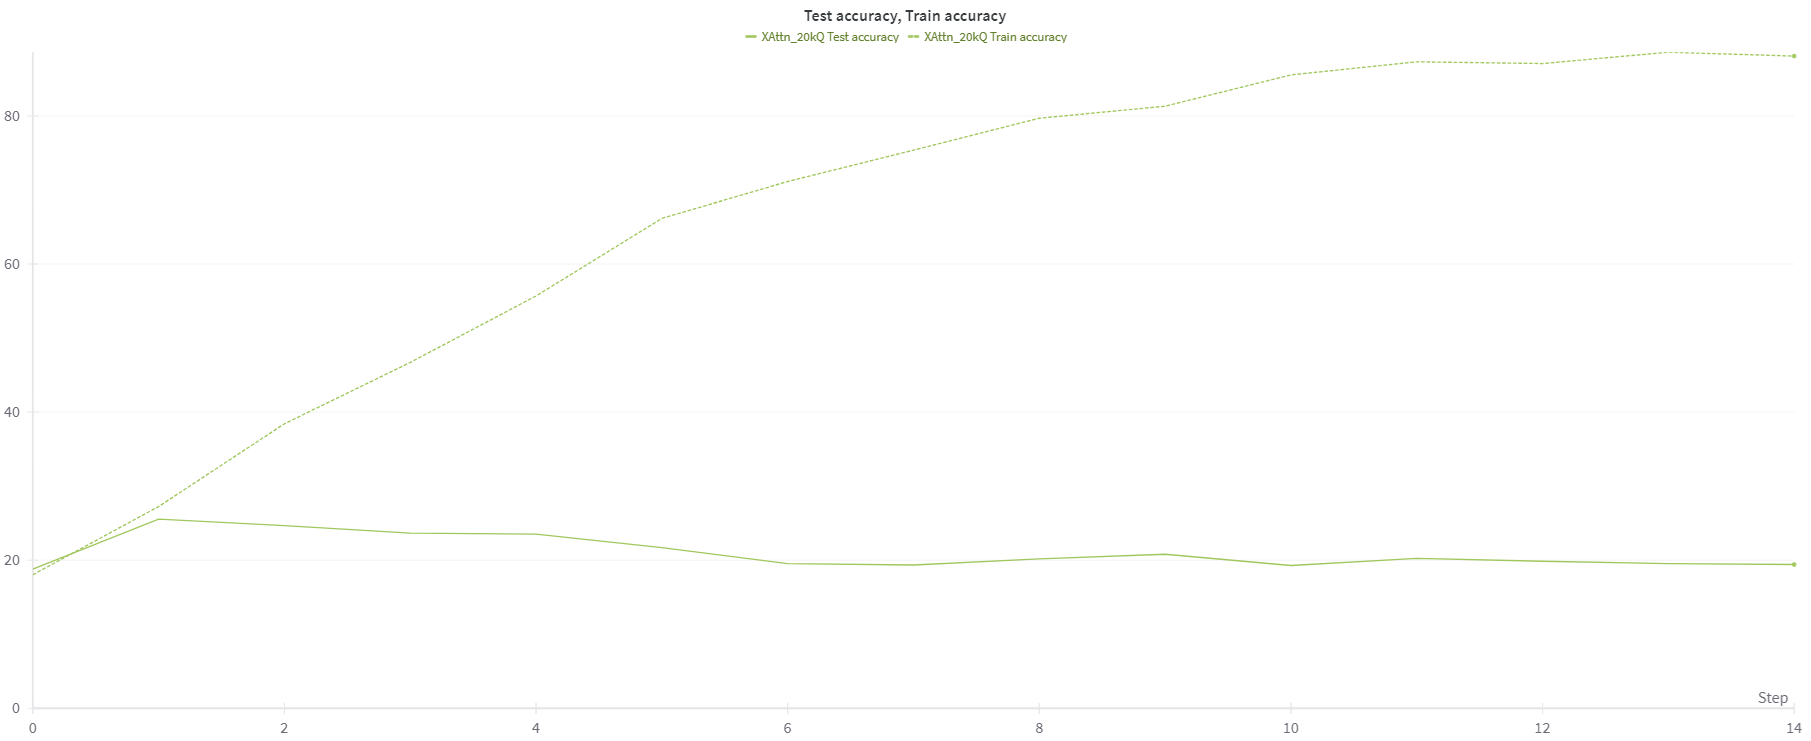
\includegraphics[width=0.4\textwidth]{images/acc.png}
%     \caption{}
%     \label{fig:example}
% \end{figure}
% \begin{figure}[h!]
%     \centering
%     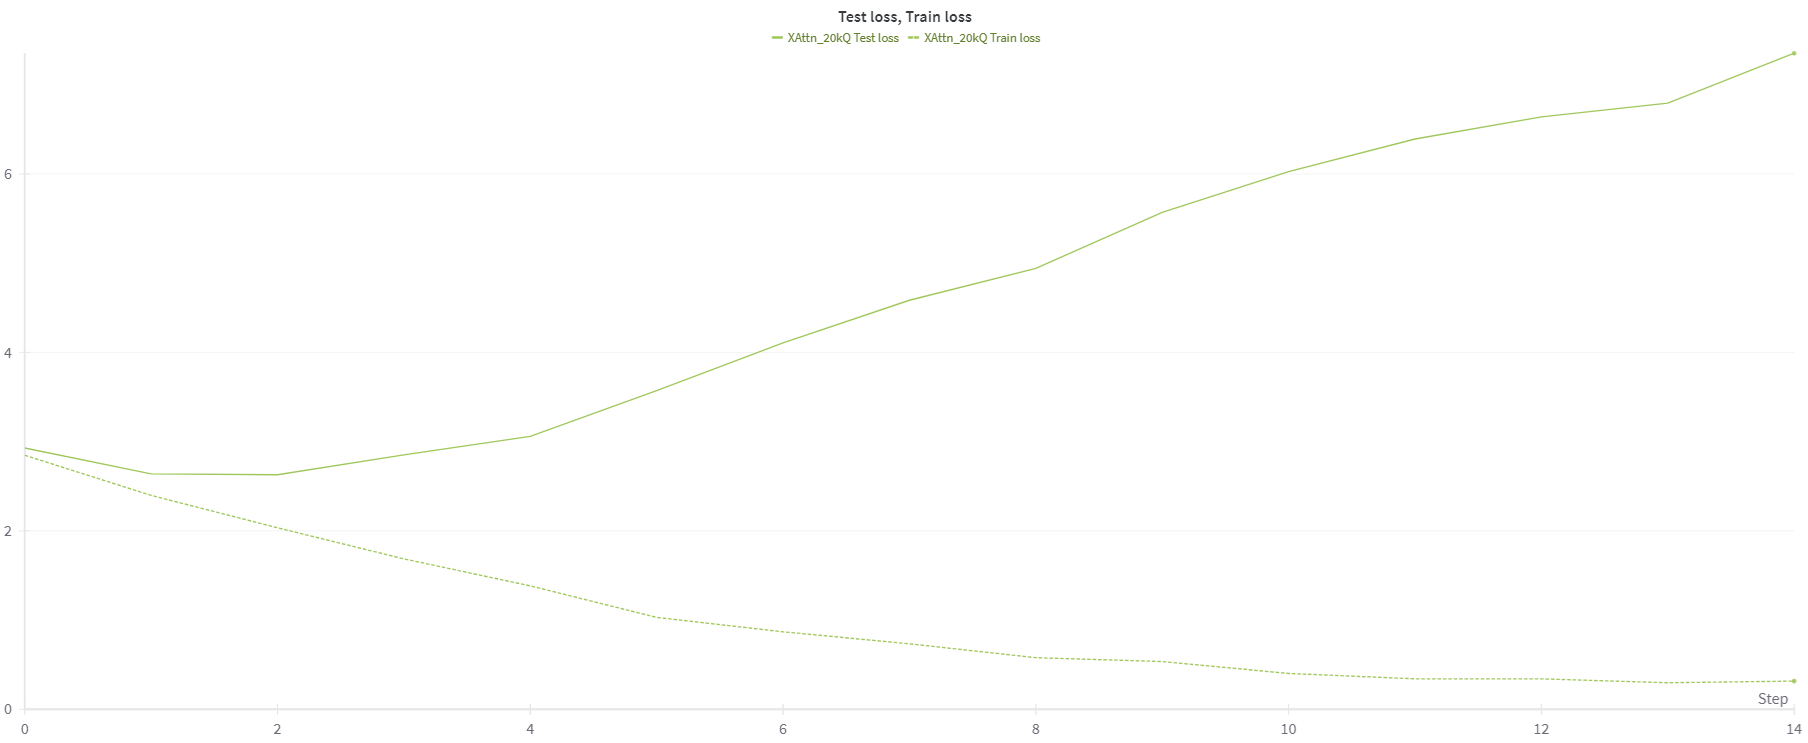
\includegraphics[width=0.4\textwidth]{images/loss.png}
%     \caption{}
%     \label{fig:example}
% \end{figure}


\subsubsection{Model Regularisation}
Overfitting is commonly caused by a model that is too complex, not regularized enough, not trained on enough data, or trained on poor quality data. To address this issue, we experiment with the following corrective approaches:
\begin{itemize}
    \item Weight decay (L2):
    \item Dropout:
    \item Increased batch size:
    \item Decreased LR:
    \item Normalization:
    \item Focal loss:
    \item Decreased model size: Number of parameters: Describe regular model (ScanSG-GNN) vs XS model (ScanSG-GNN-XS) vs. downsized model (ScanSG-GNN-32)
    \item Architectural changes: Removing some of the building blocks: Without GNN, without textencoder, with scene transformer encoder)
\end{itemize}

We retrain the ScanSG-GNN model with these changes on a smaller, $25\%$ of the dataset (5070 questions about 236 scenes). We evaluate the performance of each model with these changes on the test set of the ScanSG dataset, and report the best results in Table XXX.

\begin{table}[h!]
    \centering
    \caption{\textcolor{red}{redo these experiments if possible}}
    \begin{tabular}{l|c|}
    \cline{2-2}
                                              & \multicolumn{1}{l|}{\textbf{Test Accuracy}} \\ \hline
    \multicolumn{1}{|l|}{No changes}          & 20.1                                        \\ \hline
    \multicolumn{1}{|l|}{Batch size = 512}    & 17.9                                        \\ \hline
    \multicolumn{1}{|l|}{Weight decay = 1e-3} & 20.6                                        \\ \hline
    \multicolumn{1}{|l|}{LR = 1e-5}           & 17.5                                        \\ \hline
    \multicolumn{1}{|l|}{Normalization}       & 12.01                                       \\ \hline
    \multicolumn{1}{|l|}{Focal Loss}          & 19.0                                        \\ \hline
    \multicolumn{1}{|l|}{Dropout}             &                                             \\ \hline
    \multicolumn{1}{|l|}{XS model}            & 19.2                                        \\ \hline
    \end{tabular}
    \end{table}


We note that none of the regularization methods described above improved generalization. We therefore investigate the impact of data quality on the model's ability to generalize.

\subsection{Model Performance on Ideal Dataset}
We investigate the impact of the question dataset on model performance.
For these experiments, we split the ScanQA dataset into the following smaller datasets:

\begin{itemize}
    \item Easy dataset: contains only questions which contain the answer. Train set: 11806 questions about 555 scenes. Test set: 1083 questions about 71 scenes.
    \item Hard dataset: contains only questions which do not contain the answer. Train set: 7644 questions about 552 scenes. Test set: 498 questions about 71 scenes.
    \item Full dataset: contains all questions, same dataset as used in previous experiments.
\end{itemize}


\subsubsection{Ideal Graph Nodes, Full Question Dataset}
To understand the impact of the node embeddings on the model performance, we embed the object labels into graph nodes, rather than object images. The only difference from the previous experiment are the node embeddings. Table XX shows the results of this experiment.

\begin{table}[h!]
    \centering
    \caption{Performance on the full ScanSG+ScanQA dataset, with node embeddings computed from the object labels}
    \begin{tabular}{|l|c|l|l|l|}
    \hline
    \textbf{Model}         & \textbf{EM@1} & \textbf{EM@5} & \textbf{EM@10}  & \textbf{Sem-EM@1} \\ \hline
    Baseline               & 50.7 & 74.4 & 82.8 & 62.7 \\ \hline
    Baseline + GNN         & 16.2 & 45.3 & 62.1 & 24.7 \\ \hline
    ScanSG-GNN             & 33.1 & 73.1 & 88.0 & 43.6 \\ \hline
    ScanSG-noGNN           & \textbf{59.0} & \textbf{84.0} & \textbf{92.2} & \textbf{72.4} \\ \hline
    \end{tabular}
\end{table}

We note that results are significantly higher across all models, and the overfitting is slightly mitigated \textcolor{red}{add proof}. This shows that poor node embeddings contribute to overfitting, and low performance on the test set. The limitations of CLIP causing this were illustrated in Figure XX, and are further discussed in Section XX.
These results highlight the importance of high quality node embeddings.

The baseline outperforms the ScanSG-GNN model, and the ScanSG-noGNN is once more the best performing model.
To understand why this may be the case, we conduct the following experiments.

\subsubsection{Ideal Graph Nodes, Easy Question Dataset}

\begin{table}[h!]
    \centering
    \caption{\textcolor{red}{\textbf{Easy Q dataset Add semantic accuracy}}}
    \begin{tabular}{|l|c|l|l|l|}
    \hline
    \textbf{Model}         & \textbf{EM@1} & \textbf{EM@5} & \textbf{EM@10} & \textbf{Sem-EM@1} \\ \hline
    Baseline               & 67.3 & 91.7 & 96.6 & 83.3 \\ \hline
    Baseline + GNN         & 19.8 & 47.8 & 63.3 & 31.5 \\ \hline
    ScanSG-GNN             & 40.9 & 82.5 & 91.7 & 56.6 \\ \hline
    ScanSG-noGNN           & \textbf{76.0} & \textbf{93.6} & \textbf{97.1} & \textbf{95.0} \\ \hline
    \end{tabular}
\end{table}

results significantly higher and overfitting mitigated (show this somehow).
this method is likely better because we embed the exact label that appear in the question, so if the cross-attention mechanism works well, it just needs to select the word in the question which is also a node label.

\textcolor{red}{add attention pattern for not the best model here!! and show that the model just focuses on the matching word.}

+ and conclude that this model is good! (76) for easy input data!

\subsubsection{Ideal Graph Nodes, Hard Question Dataset}
\begin{table}[h!]
    \centering
    \caption{\textcolor{red}{\textbf{Easy Q dataset Add semantic accuracy}}}
    \begin{tabular}{|l|c|l|l|l|}
    \hline
    \textbf{Model}         & \textbf{EM@1} & \textbf{EM@5} & \textbf{EM@10} & \textbf{Sem-EM@1}\\ \hline
    ScanSG-GNN   & 24.7 & 57.6 & 72.3 & 29.7 \\ \hline
    ScanSG-noGNN & 34.9 & 62.4 & 77.9 & 43.0 \\ \hline
    \end{tabular}
\end{table}

If easy dataset is better with no-GNN because it doesnt need context awareness, maybe hard dataset can actually benefit from gnn module. so we test on hard data only and see if this is still true.

still true - 2 possible explanations for this:
- either the questions are just too hard and cant be answered (even i cant answer them tbh, there are too many possibilities)
- gnns are quite data hungry [reference] and there is not much "hard" data in this dataset. \textcolor{red}{to prove this, gradually increase datasize and show that adding more data slightly improves the proplem? maybe even do a projection of how many datapoints you would need?}

Also note that the gap between gnn and no-gnn is much smaller than in previous experiments.

todo: would be useful to take a look at which questions the gnn vs the no-gnn gets wrong.